\subsection{Módulo genérico de las rutas ferroviarias}
	\label{sec:ACG_rts}
	
	El módulo \textit{Routes} (ver Figura \ref{fig:GeneralSystem}) es el encargado de implementar el funcionamiento de las rutas ferroviarias. El ACG determina todos los elementos ferroviarios que abarca la ruta e implementa los puertos y conexiones a cada uno de estos elementos. De esta manera, cada módulo \textit{Routes} tiene la información necesaria del estado actual de cada elemento y si se encuentran o no enclavados. Además, el ACG implementa las salidas necesarias para consultar y controlar cada elemento ferroviario en cuestión, junto con la dinámica interna para determinar si la ruta puede ser habilitada y bajo que condiciones. El diagrama de bloques de la máquina de estados finitos con camino de datos diseñado para lograr este objetivo se muestra en la Figura \ref{fig:RTS_module}.
	
	\begin{figure}[H]
		\centering
		\includegraphics[width=1\textwidth]{Figuras/RTS_module}
		\centering\caption{FSMD del módulo genérico de \textit{Routes}}
		\label{fig:RTS_module}
	\end{figure}
	
	Inicialmente, el módulo \textit{Routes} se encuentra inactivo, esperando que la ruta sea solicitada por el operador. De recibir la orden esperaba, el módulo comprobará que todos los \textit{netElements} se encuentran liberados (ni reservados ni enclavados por otras rutas) y libres (no ocupados por ninguna formación). De ser afirmativa la respuesta, se enviará la señal de reserva y de confirmarse la reserva, se envía la señal de enclavamiento a los \textit{netElements}. Estos pasos deberán hacerse dentro de un intervalo de tiempo determinado o el pedido de ruta será cancelado.
	
	A continuación, una vez se confirma que toda la sección está enclavada, se repite el procedimiento de verificación de estado, reserva y enclavamiento con cada elemento ferroviario necesario para asegurar la ruta. Si alguno de estos elementos no se encuentra disponible, la ruta es cancelada por timeout y todas las secciones y componentes previamente enclavados son liberados. Si todas las condiciones de ruta son satisfechas, la ruta es habilitada y se toma el control de la señal inicial.El comportamiento de las rutas ferroviarias se define en la red de Petri de la Figura \ref{fig:RTS_Petri}.
	
	\begin{figure}[H]
		\centering
		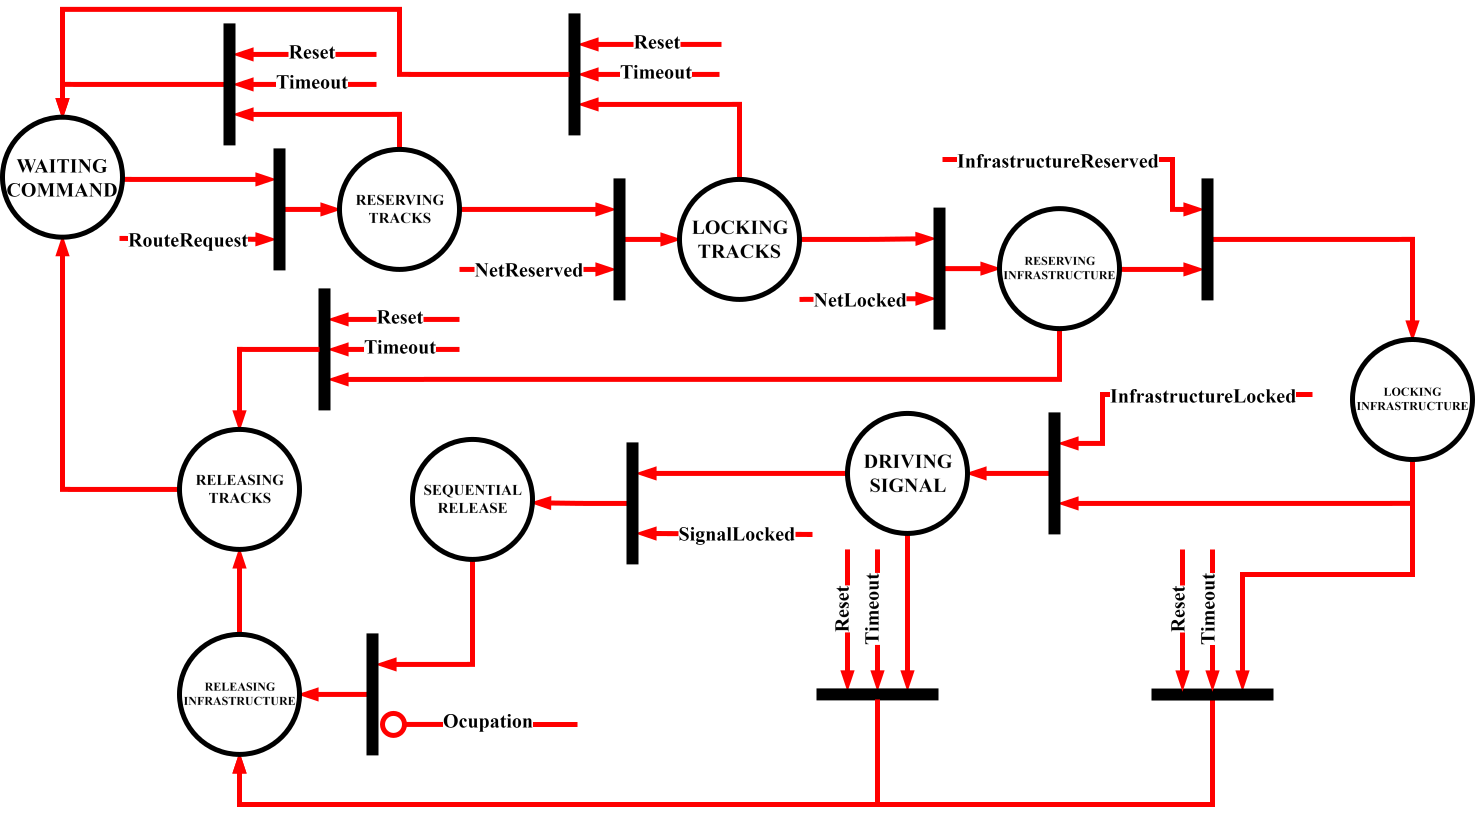
\includegraphics[width=1\textwidth]{Figuras/RTS_petri}
		\centering\caption{Red de Petri del modelo dinámico de \textit{Routes}.}
		\label{fig:RTS_Petri}
	\end{figure}
	
	A medida que la formación va circulando se activa la liberación secuencial de los elementos ferroviarios dejados atrás por la formación, lo cual permite una mayor flexibilidad a la hora de asignar y liberar rutas, como se explicó en la Sección \ref{sec:ACG_liberacion}. Al finalizar la liberación secuencial, si la formación ya no ocupa ninguna sección de la ruta, entonces se procede a liberar los elementos restantes y la ruta vuelve a su estado de espera inicial.
	
	Las rutas no comprueban el estado de rutas antagónicas ni rutas con las que compartan recursos, solamente sus propias condiciones de habilitación. Esto es así ya que se delegó en cada elemento la facultad de ser reservados y enclavados por una única ruta, lo cual impide la existencia de rutas conflictivas habilitadas simultáneamente. De otra manera, las rutas usarían demasiados recursos mientras que los elementos ferroviarios muchos menos. Una distribución de las responsabilidades otorga mas flexibilidad y escalabilidad al sistema, con módulos de similares tamaños y complejidad.